\documentclass[a4paper,12pt]{article}

% Paquetes básicos
\usepackage[utf8]{inputenc}
\usepackage[T1]{fontenc}
\usepackage[spanish]{babel}
\usepackage{graphicx}
\usepackage{xcolor}
\usepackage{lipsum}
\usepackage{geometry}
\geometry{top=3cm, bottom=3cm, left=2.5cm, right=2.5cm}

% Paquetes para diseño
\usepackage{titlesec}
\usepackage{fancyhdr}
\usepackage{amsmath}
\usepackage{amssymb}
\usepackage{hyperref}

\usepackage{tikz} 
\usetikzlibrary{shapes.geometric, arrows} 
\tikzstyle{startstop} = [rectangle, rounded corners, minimum width=3cm, minimum height=1cm,text centered, draw=black] \tikzstyle{process} = [rectangle, minimum width=3cm, minimum height=1cm, text centered, draw=black] 
\tikzstyle{arrow} = [thick,->,>=stealth]

% Paquetes para el entorno lstlisting
\usepackage{listings}


\usepackage{inconsolata}

% Paquete para fondo
\usepackage{background}

% Configuración de lstlisting
\lstset{
    inputencoding=utf8,          % Permite UTF-8
    extendedchars=true,          % Reconoce caracteres extendidos
    literate=                    % Configuración manual para tildes y símbolos
        {á}{{\'a}}1
        {é}{{\'e}}1
        {í}{{\'i}}1
        {ó}{{\'o}}1
        {ú}{{\'u}}1
        {ñ}{{\~n}}1
        {Á}{{\'A}}1
        {É}{{\'E}}1
        {Í}{{\'I}}1
        {Ó}{{\'O}}1
        {Ú}{{\'U}}1
        {Ñ}{{\~N}}1
        {¿}{{\textquestiondown}}1
        {¡}{{\textexclamdown}}1,
    basicstyle=\ttfamily,        % Fuente monoespaciada
    breaklines=true,             % Habilita salto de línea automático
    frame=single,                % Marco alrededor del código
    backgroundcolor=\color{gray!10}, % Fondo gris claro
    keywordstyle=\color{blue},   % Color para palabras clave
    commentstyle=\color{green},  % Color para comentarios
    stringstyle=\color{red}      % Color para strings
}
\lstdefinestyle{customcpp}{
    language=C++,                % Lenguaje de programación
    showspaces=false,            % No mostrar espacios
    showtabs=false,              % No mostrar tabulaciones
    tabsize=4,                   % Tamaño de tabulación
    showstringspaces=false,      % No mostrar espacios en strings
    numbers=left,                % Números de línea a la izquierda
    numberstyle=\tiny\color{gray}, % Estilo de los números de línea
    numbersep=5pt,               % Separación de los números de línea
    stepnumber=1,                % Mostrar número en cada línea
    basicstyle=\ttfamily\footnotesize, % Estilo básico del código
    keywordstyle=\bfseries\color{blue}, % Estilo de las palabras clave
    commentstyle=\itshape\color{green!50!black}, % Estilo de los comentarios
    stringstyle=\color{red},     % Estilo de los strings
    identifierstyle=\color{black}, % Estilo de los identificadores
    % procnamekeys={def,class},    % Palabras clave para nombres de funciones
    morekeywords={constexpr,nullptr,size_t}, % Más palabras clave
    emph={int,char,double,float,unsigned}, % Palabras a enfatizar
    emphstyle=\color{magenta},   % Estilo de las palabras enfatizadas
    backgroundcolor=\color{gray!10}, % Color de fondo
    frame=shadowbox,             % Marco con sombra
    rulesepcolor=\color{gray},   % Color de la línea de separación
    breakatwhitespace=false,     % No cortar en espacios en blanco
    breaklines=true,             % Cortar líneas largas
    captionpos=b,                % Posición del título (abajo)
    escapeinside={(*@}{@*)},     % Delimitadores para escapar a LaTeX
    morecomment=[l][\color{magenta}]{\#}, % Comentarios de una línea
    morecomment=[s][\color{orange}]{/*}{*/}, % Comentarios multilínea
    morestring=[b]",             % Strings entre comillas dobles
    morestring=[b]'              % Strings entre comillas simples
}

% Configuración de título
\titleformat{\section}{\normalfont\Large\bfseries}{\thesection}{1em}{}

% Información del documento
\title{
    \vspace{-2cm}
    
\includegraphics[width=0.2\textwidth]{images/etsiit.png} \\ % Cambia el logo si es necesario
    \LARGE \textbf{Algoritmo de la Criba de Eratóstenes usando MPI (Message Passing Interface)} \\[0.5cm]
    \large \textbf{Sistemas Concurrentes y Distribuidos} \\[0.5cm]}
\author{
    \textbf{Ismael Sallami Moreno} \\
    \textit{Ingenería Informática + ADE} \\
    \textit{Universidad de Granada (UGR)} \\
}
\date{\today}

% Configuración del fondo
\backgroundsetup{
    scale=1,
    color=black,
    opacity=0.2,
    angle=0,
    position=current page.south,
    vshift=0pt,
    hshift=0pt,
    %contents={\includegraphics[width=\paperwidth,height=\paperheight,keepaspectratio]{images/Eratóstenes1.jpg}}
}

%pon el customc del estilo de lstlisting
\lstset{style=customcpp}

% Inicio del documento
\begin{document}

% Portada
\maketitle
\thispagestyle{empty}

% \begin{center}
%     \includegraphics[width=\textwidth,height=0.4\textheight,keepaspectratio]{images/Eratóstenes1.jpg} \\ % Añade tu imagen de fondo
%     \vfill
% \end{center}

\newpage

% Índice (opcional)
\tableofcontents
\newpage

\section{Enunciado de la Actividad}

El objetivo de este ejercicio es programar una versión distribuida del famoso método de \textit{la criba de Erastotenes} para obtener los \(N\) primeros números primos. Se utilizará una red de procesos concurrentes conectados por una tubería o "pipeline" de procesos, como en la figura siguiente, para generar los \(N\) primeros números primos.

% \begin{figure}[h!]
%     \centering
%     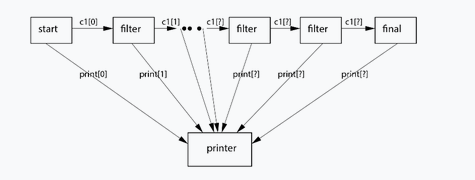
\includegraphics[width=\textwidth]{images/pipeline.png}
%     \caption{Pipeline de procesos para generar números primos}
% \end{figure}
\begin{figure}[h!]
    \centering
    \begin{tikzpicture}[node distance=2cm, scale=0.8, transform shape]
        \node (start) [startstop] {start};
        \node (filter1) [process, right of=start, xshift=2cm] {filter};
        \node (filter2) [process, right of=filter1, xshift=2cm] {filter};
        \node (filter3) [process, right of=filter2, xshift=2cm] {filter};
        \node (filter4) [process, right of=filter3, xshift=2cm] {filter};
        \node (final) [startstop, right of=filter4, xshift=2cm] {final};
        \node (printer) [process, below of=filter2, yshift=-2cm] {printer};
        
        \draw [arrow] (start) -- node[anchor=south] {c1[0]} (filter1);
        \draw [arrow] (filter1) -- node[anchor=south] { c1[1]} (filter2);
        \draw [arrow] (filter2) -- node[anchor=south] {\dots} (filter3);
        \draw [arrow] (filter3) -- node[anchor=south] {c1[?]} (filter4);
        \draw [arrow] (filter4) -- node[anchor=south] {c1[?]} (final);
        \draw [arrow] (start) -- node[anchor=east] {print[0]} (printer);
        \draw [arrow] (filter1) -- node[anchor=east] {print[1]} (printer);
        \draw [arrow] (filter2) -- node[anchor=east] {print[?]} (printer);
        \draw [arrow] (filter3) -- node[anchor=east] {print[?]} (printer);
        \draw [arrow] (filter4) -- node[anchor=east] {print[?]} (printer);
        \draw [arrow] (final) -- node[anchor=east] {print[?]} (printer);
    \end{tikzpicture}
    \caption{Pipeline de procesos para generar números primos}
\end{figure}


Para programarlo, suponer que se conoce una constante \texttt{nLimite} que es mayor o igual que el \(N\)-ésimo número primo. El proceso \texttt{start} generará el primer número primo (el 2) y lo enviará al proceso \texttt{printer}, que lo imprime; a continuación genera el siguiente primo (el 3), lo envía al primer proceso \texttt{filter}, al que seguirá enviando los siguientes números impares: 5, 7, 9, y así sucesivamente. 


\section{Solución con MPI}

La solución propuesta consiste en ejecutar el programa de la criba de Eratóstenes utilizando MPI. A medida que se incrementa el número de procesos especificados con `mpirun`, se añaden más filtros, lo que mejora la precisión y eficiencia del resultado.

\lstinputlisting{../criba.cpp}

\subsection{Explicación detallada del código}

El código presentado implementa la criba de Eratóstenes utilizando \textit{MPI} (Message Passing Interface) para calcular números primos de forma concurrente y distribuida. A continuación, se describen las funciones principales de cada bloque del programa:

\subsubsection{Inicialización y configuración}
El programa comienza inicializando el entorno de ejecución con \texttt{MPI\_Init}, obteniendo el rango (\texttt{rank}) y el tamaño (\texttt{size}) del comunicador global \texttt{MPI\_COMM\_WORLD}. Si el número de procesos es menor que 3, el programa imprime un mensaje de error y aborta la ejecución mediante \texttt{MPI\_Abort}. Esto asegura que haya al menos un generador, un filtro y un impresor.

\subsubsection{Generador de números (Proceso 0)}
El proceso con \texttt{rank = 0} actúa como generador de números naturales. Inicialmente, envía el número 2 (el primer número primo) directamente al impresor (\texttt{rank = size - 1}). Luego, comienza un bucle que genera números naturales secuenciales. Cada número se envía al primer filtro (\texttt{rank = 1}) usando \texttt{MPI\_Send}.

El generador finaliza cuando el número actual supera el límite predefinido (\texttt{nLimite}). En ese momento, envía una señal especial de terminación (\texttt{x = -1}) al primer filtro.

\subsubsection{Filtros intermedios (Procesos con $1 \leq \texttt{rank} < \texttt{size} - 1$)}
Cada filtro intermedio tiene la responsabilidad de descartar números que no son primos. El primer número recibido por un filtro se considera su número primo característico (\texttt{primo}). 

Los filtros reciben números desde el proceso anterior mediante \texttt{MPI\_Recv}. Si el número recibido no es divisible por \texttt{primo}, el filtro lo reenvía al siguiente filtro usando \texttt{MPI\_Send}. Si el filtro detecta la señal de terminación (\texttt{x = -1}), la propaga al siguiente proceso y termina su ejecución.

Este diseño asegura que cada filtro actúe como un módulo de exclusión para números no primos, delegando la validación de números más grandes a los filtros siguientes.

\subsubsection{Impresor de números primos (Último proceso)}
El proceso con \texttt{rank = size - 1} es responsable de imprimir los números primos. Recibe números desde el último filtro intermedio y los imprime en pantalla. Al recibir la señal de terminación (\texttt{x = -1}), el impresor detiene su ejecución.

\subsubsection{Finalización del programa}
Todos los procesos llaman a \texttt{MPI\_Finalize} para limpiar el entorno de ejecución de MPI y asegurar una terminación ordenada.




\subsection{Compilación}

\lstinputlisting{../comandoEjecucion.txt}

\subsection{Ejecución y/o salida }
\subsubsection{Con 3 procesos}
\lstinputlisting{../salida3.txt}

\subsubsection{Con 4 procesos}
\lstinputlisting{../salida4.txt}

\subsubsection{Con 5 procesos}
\lstinputlisting{../salida5.txt}

\subsubsection{Con 10 procesos}
\lstinputlisting{../salida10.txt}
\subsubsection{Con 20 procesos}
\lstinputlisting{../salida20.txt}

\subsubsection{Justificación del comportamiento según el número de procesos}

El comportamiento del programa varía significativamente dependiendo del número de procesos utilizados en la ejecución. Este fenómeno puede explicarse en términos de cómo los procesos filtran números no primos y cómo se organiza la comunicación entre ellos.

\paragraph{Con un menor número de procesos (por ejemplo, 3):}
Cuando el número de procesos es bajo, la cantidad de filtros disponibles es insuficiente para eliminar todos los números compuestos (no primos). Por ejemplo, con 3 procesos:
\begin{itemize}
    \item El primer proceso (\texttt{rank = 1}) filtra números divisibles por 2.
    \item El segundo proceso (\texttt{rank = 2}) filtra números divisibles por 3.
\end{itemize}
Sin embargo, no hay suficientes procesos para filtrar números compuestos mayores, como los divisibles por 5, 7, etc. Como resultado, algunos números no primos pasan a través del sistema y son enviados al impresor. Esto genera una salida con más números, pero no todos son primos.

\paragraph{Con un mayor número de procesos:}
A medida que se incrementa el número de procesos, se añaden más filtros, cada uno dedicado a eliminar los números divisibles por un número primo específico. Por ejemplo:
\begin{itemize}
    \item Un proceso adicional (\texttt{rank = 3}) filtra los números divisibles por 5.
    \item Otro proceso (\texttt{rank = 4}) filtra los números divisibles por 7.
\end{itemize}
Con más procesos, los números compuestos tienen más probabilidades de ser eliminados antes de llegar al impresor, lo que garantiza que la salida sea exclusivamente números primos. Sin embargo, este aumento de precisión también implica que se procesen menos números, ya que cada filtro elimina una mayor cantidad de candidatos.


\subsection{Demostración Matemática de la Correctitud del Algoritmo}

El algoritmo implementado se basa en la Criba de Eratóstenes, un método clásico para encontrar números primos en un rango dado. A continuación, demostramos matemáticamente que este enfoque es correcto.

\subsubsection{Definición de Número Primo}

Un número \( n > 1 \) es primo si y solo si no es divisible por ningún número entero \( k \) tal que \( 2 \leq k \leq \sqrt{n} \). Es decir, no existen divisores propios de \( n \) en el rango mencionado.

\subsubsection{Esquema del Algoritmo}

El algoritmo utiliza un conjunto de procesos para filtrar números no primos de manera iterativa:
\begin{enumerate}
    \item El primer proceso (\texttt{rank == 0}) genera números consecutivos \( x \) comenzando desde 2 y los envía al primer filtro.
    \item Cada proceso filtro \( P_i \) conserva un número primo \( p_i \), recibido del proceso anterior. Filtra los números \( x \) recibidos eliminando aquellos que satisfacen \( x \mod p_i = 0 \) (es decir, los múltiplos de \( p_i \)).
    \item Los números que no son múltiplos de \( p_i \) son enviados al siguiente filtro.
    \item Finalmente, el último proceso (\texttt{rank == size - 1}) imprime todos los números que llegan hasta él, ya que no han sido descartados por ningún filtro previo.
\end{enumerate}

\subsubsection{Correctitud del Algoritmo}

Para demostrar que este algoritmo es correcto, debemos probar que:

\begin{enumerate}
    \item \textbf{Todo número primo es identificado correctamente.}
    \item \textbf{Todo número compuesto es eliminado correctamente.}
\end{enumerate}

\paragraph{Identificación de números primos}

Por definición, un número primo \( p \) no tiene divisores propios en el rango \( [2, \sqrt{p}] \). En el algoritmo:
\begin{itemize}
    \item El primer filtro retiene \( 2 \), el siguiente retiene \( 3 \), y así sucesivamente.
    \item Un número \( p \) que llega al filtro \( P_i \) no es divisible por \( p_1, p_2, \ldots, p_{i-1} \), ya que estos filtros han descartado previamente los múltiplos de sus primos asociados.
    \item Si \( p \) llega al último filtro, entonces \( p \) no tiene divisores en \( [2, \sqrt{p}] \), lo que implica que es primo.
\end{itemize}

Por lo tanto, el algoritmo identifica todos los números primos correctamente.

\paragraph{Eliminación de números compuestos}

Sea \( n \) un número compuesto. Por definición, \( n \) tiene al menos un divisor \( d \) tal que \( 2 \leq d \leq \sqrt{n} \). En el algoritmo:
\begin{itemize}
    \item El filtro correspondiente al primo \( d \) descarta \( n \), ya que \( n \mod d = 0 \).
    \item Como \( d \leq \sqrt{n} \), el filtro asociado a \( d \) se encuentra antes de los procesos que manejan \( n \), asegurando su eliminación.
\end{itemize}

Por lo tanto, ningún número compuesto llega al último proceso impresor.

\subsubsection{Conclusión del Análisis}

El algoritmo implementado en MPI garantiza que:
\begin{itemize}
    \item Todos los números primos dentro del rango son impresos.
    \item Ningún número compuesto es identificado como primo.
\end{itemize}

Esto demuestra matemáticamente que el algoritmo es correcto y cumple con los requisitos de la Criba de Eratóstenes para la identificación de números primos, por lo tanto queda demostrado el algoritmo de la Criba de Eratóstenes.

\end{document}
